%\chapter*{Введение}
%\addcontentsline{toc}{chapter}{Введение}

\newpage
\begin{center}
\textbf{ГЛАВА 1}\\
\textbf{Основные физические свойства коллоидных систем}
\end{center}
\refstepcounter{chapter}


% \section*{}
\addcontentsline{toc}{chapter}{ГЛАВА 1. Основные физические свойства коллоидных систем}


\section{Типы взаимодействий частиц}\label{C1_1}
Каждое вещество имеют свою внутреннюю структуру, которая определяет его физические свойства. Вещество состоит из частиц, которые представляют собой материальные точки, они моделируют атомы и молекулы в молекулярных системах. Взаимодействие частиц описывается посредством потенциалов взаимодействия, основным свойством которых является отталкивание при сближении и притяжение при удалении. Методом динамики частиц можно моделировать эффекты разрушения, пластичность, температурное изменение свойств материала, фазовые переходы [1].

Широкий круг проблем физики связан с системами с дальнодействующими взаимодействиями. Однако их статистические и динамические свойства гораздо менее понятны, чем у систем с малым радиусом действия [2]. Примеры дальнодействующих взаимодействий можно найти в астрофизике, физике плазмы, гидродинамике, в атомной физике и ядерной физике. Это повсеместное присутствие в различных физических дисциплинах само по себе оправдывает необходимость общего и междисциплинарного понимания физических и математических проблем, возникающих в системах взаимодействия на больших расстояниях. 

Определим, какое свойство взаимодействий делает его короткодействующим или дальнодействующим. Для достаточно больших расстояний $r$ абсолютное значение потенциала двух тел ограничено $r^{-\alpha}$. Если положительная степень $\alpha$ больше, чем размерность пространства d, в которое встроена система, $\alpha>d$, мы определяем систему как короткодействующую. В противном случае, если $\alpha \leq d$, система является дальнодействующей.

К дальнодействующим взаимодействиям относят электростатические взаимодействия между ионами, металлическую связь и силы Ван-дер-Ваальса. 

\textbf{Радиус действия} – это максимальное расстояние между частицами, за пределами которого их взаимодействием можно пренебречь.

Сильное и слабое взаимодействия являются короткодействующими. Их интенсивность быстро убывает при увеличении расстояния между частицами.  Электромагнитное и гравитационное взаимодействия являются дальнодействующими. Такие взаимодействия медленно убывают при увеличении расстояния между частицами и не имеют конечного радиуса действия.

К межмолекулярным взаимодействиям относятся взаимодействия между молекулами и/или атомами, не приводящие к образованию ковалентных химических связей.

Межмолекулярные взаимодействия имеют электростатическую природу. На больших расстояниях преобладают силы притяжения, которые могут иметь ориентационную, поляризационную и дисперсионную природу.

Модельными системами называют системы, в которых микроскопические частицы выступают в роли атома или молекул [1]. Главными особенностями таких систем является возможность регулирования взаимодействия между частицами посредством внешних параметров, например: внешнее электрическое поле, внешнее магнитное поле, тепловое и другие. Известными примерами модельных систем являются пылевая плазма и коллоидные системы. 

Твердые частицы размером от десятков нанометров до десятков микрометров, погруженные в сольвент, называют коллоидной системой или дисперсией.

В пылевой плазме реализуется чисто отталкивающее взаимодействие между частицами [3]. Это накладывает некоторые ограничения на спектр исследуемых явлений. Коллоидные системы с точки зрения взаимодействия являются более гибким инструментом. Сами по себе коллоидные частицы обладают лишь отталкивающим взаимодействием, однако при наличии внешних полей возникает и притягивающая ветвь. Наличие притяжения позволяют изучать широкий класс явлений: нуклеацию, спинодальный распад, кристаллизацию, плавление, движение дислокаций, фазовые переходы кристалл-кристалл, жидкость-газ.

Как правило, из-за разного материала частиц и сольвента возникает притяжение Ван-дер-Ваальса \cite{Yur31, Yur53}:
\begin{equation}
\varphi_{\mathrm{vdW}}(r)=-\frac{A_{\mathrm{H}}}{12}\left(\frac{\sigma^{2}}{r^{2}-\sigma^{2}}+\frac{\sigma^{2}}{r^{2}}+2 \ln \frac{r^{2}-\sigma^{2}}{r^{2}}\right)
\end{equation}
где постоянная Хамакера $A_{\mathrm{H}} \propto\left(\frac{\varepsilon_{\mathrm{r}}-1}{\varepsilon_{\mathrm{r}}+1}\right)^{2}$ зависит от относительной диэлектрической проницаемости $\varepsilon_{\mathrm{r}}=\varepsilon_{\mathrm{P}} / \varepsilon_{\mathrm{S}}$. 

Для предотвращения коагуляции в коллоидной системе присутствуют силы отталкивания, которые обусловлены зарядовой или стерической стабилизацией.

Зарядовая стабилизация возникает благодаря взаимному отталкиванию заряженных частиц, в результате накопленного на их поверхности отрицательного заряда, который возникает при диссоциации поверхности и адсорбции ионов. 
В рамках линеаризованной теории Пуассона-Больцмана, взаимодействие Дерягина-Ландау-Фервея-Овербека имеет вид \cite{Yur54}
\begin{equation}
\varphi_{Y}(r)=\left\{\begin{array}{ll}
\infty & r<\sigma, \\
\epsilon_{\mathrm{Y}} \frac{e^{-\kappa(r-\sigma)}}{r / \sigma} & r \geq \sigma,
\end{array}\right.
\end{equation}

где $\kappa=\sqrt{4 \pi \lambda_{\mathrm{B}} n_{\mathrm{ion}}} \equiv \lambda_{\mathrm{D}}^{-1}$ - обратная дебаевская длина экранирования, выраженная через плотность малых ионов $n_{ion}$ и длину Бьеррума $\lambda_{\mathrm{B}}=e^{2} / \varepsilon_{\mathrm{w}} k_{\mathrm{B}} T$. Контактный потенциал записывается как 

\begin{equation}
\epsilon_{\mathrm{Y}}=\frac{Z^{2}}{(1+\kappa \sigma / 2)^{2}} \frac{\lambda_{\mathrm{B}}}{\sigma} k_{\mathrm{B}} T,
\end{equation}
где $Z \equiv Q / e$ зарядовое число коллоида.

Результирующее взаимодействие представляет собой сумму притягивающих и отталкивающих сил:
\begin{equation}
\varphi(r)=\varphi_{Y}(r)+\varphi_{\mathrm{vdW}}(r).
\end{equation}
Вклады данных слагаемых соизмеримы на малом расстоянии между не сильно заряженными частицами.

С ростом заряда частиц, теория Пуассона-Больцмана становится неприменимой вблизи поверхности частицы, однако на дальних расстояния по прежнему имеет форму Юкавы, и при ренормированном зарядом может хорошо описывать потенциал вдали от поверхности \cite{Yur55}. Эффективный насыщенный заряд выражается следующим уравнением \cite{Yur56}
\begin{equation}
Z_{\mathrm{eff}}^{\mathrm{sat}}=(2+\kappa \sigma) \sigma / \lambda_{\mathrm{B}}
\end{equation}
Используя линеаризованную теорию Пуассона - Больцмана с установленным эффективным зарядом, можно объяснить большинство экспериментальных наблюдений \cite{Yur57, Yur58, Yur59}. Это делает теорию Дерягина-Ландау-Фервея-Овербека (ДЛФО) одним из наиболее успешных подходов при описании межчастичных взаимодействий \cite{Yur49, Yur60, Yur61}. 

Помимо зарядовой стабилизации существует так называемая стерическая стабилизация. Она заключается в добавлении в сольвент полимерных молекул, которые оседают на частицах. При сближении частиц, эти полимерные цепи взаимодействуют друг с другом, не давая частицам сблизиться сильнее. 

\begin{figure}[!h]
\begin{center}
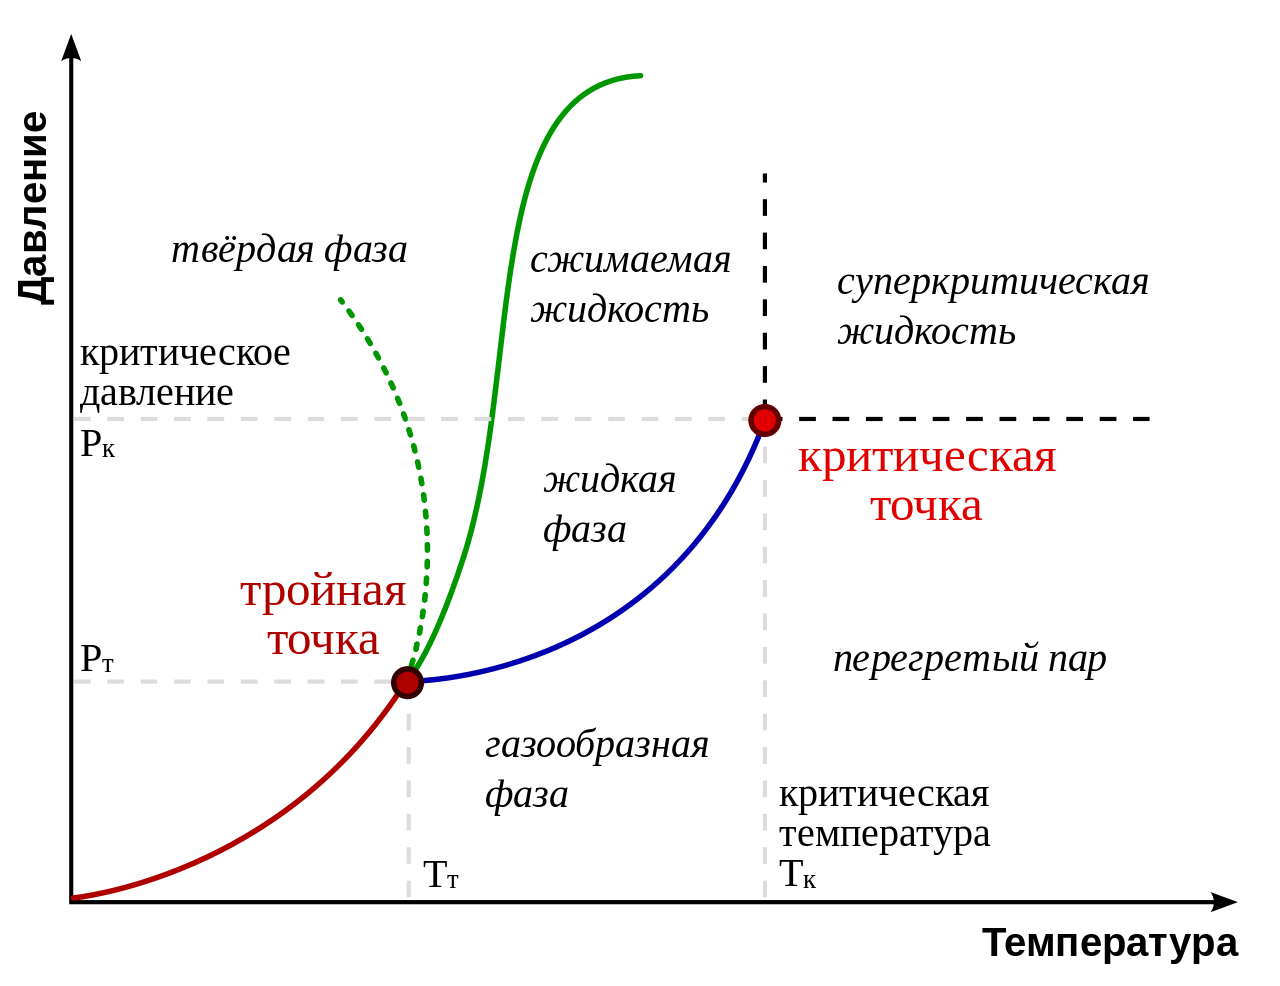
\includegraphics[width=0.75\textwidth]{1280px-Phase-diag_ru.svg.png}
\caption{Виды фазовых диаграмм. Зеленая линия - аномальное поведение воды.}
\label{част}
\end{center}
\end{figure}

\section{Модельные потенциалы взаимодействий}
Потенциал взаимодействия – характеристика, определяющая термодинамику системы. Понимание, как зависит потенциал от внешних параметров, позволяет управлять взаимодействием между частицами. Это дает возможность изменять групповое поведение в системе. Первый вариант- можно увеличивать или уменьшать притягивающую или отталкивающую ветвь, т.е. контролировать размер и количество агломератов в системе. Второй вариант - можно создать чисто отталкивающий потенциал. Потенциал взаимодействия играет важную роль в динамике частиц. Конкретный вид потенциала взаимодействия частиц определяется, исходя из сравнения механических свойств компьютерного и реального материалов. Для правильного описания механических свойств материала при компьютерном моделировании параметры потенциала взаимодействия необходимо задавать в соответствии с введенным радиусом обрезания. Регулировка потенциала может осуществляться с помощью внешних полей: тепловых, химических, магнитных и электрических. Она происходит за счет изменения амплитуды поля, таким образом можно контролировать величину индуцированного заряда, величину намагниченности или величину градиентных сил, а значит и взаимодействие. 
 
Многие модельные системы, используемые для экспериментов с разрешением частиц, такие как коллоидные суспензии и сложные (пыльные) плазмы, парные взаимодействия на коротких расстояниях в основном описываются отталкиванием Юкавы [4].

Система точечных частиц в 2D геометрии, взаимодействует через попарно отталкивающий потенциал вида:
\begin{equation}
\varphi(r)=\frac{\varepsilon \lambda}{r} \exp \left(-\frac{r}{\lambda}\right)
\end{equation}

где $\varepsilon, \lambda$ - энергетические и экранирующие масштабы длин взаимодействия. Для заряженных частиц, погруженных в плазмоподобную экранирующую среду, энергетическая шкала равна:
\begin{equation}
\varepsilon=Q^{2} / 4 \pi \epsilon_{0} \lambda
\end{equation}

где $Q$ - заряд, $\epsilon_{0}$ - диэлектрическая проницаемость пространства.

Свойства систем Юкавы определяются двумя параметрами: параметром связи и параметром отбора. Первый определяется так:
\begin{equation}
\text{Г}=Q^{2} / 4 \pi \epsilon_{0} a k_{\mathrm{B}} T
\end{equation}

где $k_b$ - постоянная Больцмана, T - температура, $a=(\pi n)^{-1 / 2}$ - радиус Вигнера-Зейтца, где n - концентрация частиц на единицу объема.

Второй параметр равен:
\begin{equation}\kappa=a / \lambda\end{equation}

Заметим, что параметр связи - отношение потенциальной энергии взаимодействия двух соседних частиц к их кинетической энергии. Обычно говорят, что система находится в сильно связанном состоянии, когда это соотношение велико [4].

Часть потенциала взаимодействия, которая соответствует стерической стабилизации, выглядит следующим образом \cite{Yur31}
\begin{equation}
\begin{array}{l}
\varphi_{\text {steric }}(r)=\frac{\pi \sigma}{2} \int_{r-\sigma}^{\infty} d h F(h) \\
\\
F(r)=\frac{\alpha k_{\mathrm{B}} T}{s^{3}}\left[\left(\frac{2 L}{r}\right)^{9 / 4}-\left(\frac{r}{2 L}\right)^{3 / 4}\right], \quad r<2 L
\end{array}
\label{eqStericStabl}
\end{equation}
где $L$ - толщина полимерного слоя, $\alpha$ - численный множитель, определяемый для конкретных полимеров
особенностями взаимодействия между молекулярными цепочками, $s$ - среднее расстояние между привитыми полимерами на поверхности.

В случае наличия этих взаимодействий, суммарный потенциал частиц выражается следующей формулой

\begin{equation}
\varphi(r)=\varphi_{Y}(r)+\varphi_{\mathrm{vdW}}(r)+\varphi_{\mathrm{steric}}(r).
\end{equation}

Для изучения влияния микроскопических свойств на макроскопические свойства, используется так называемый метод молекулярной динамики, который заключается в численном моделировании системы, состоящей из достаточно большого количества частиц, по статистике которых можно судить о макроскопических свойствах. Одним из наиболее популярных модельных потенциалов взаимодействия частиц в таких системах, является потенциал Леннарда - Джонса:
\begin{equation}
U\left(R_{i j}\right)=\varepsilon\left[\left(\frac{R_{0}}{R_{i j}}\right)^{12}-2\left(\frac{R_{0}}{R_{i j}}\right)^{6}\right]=4 \varepsilon\left[\left(\frac{\sigma}{R_{i j}}\right)^{12}-\left(\frac{\sigma}{R_{i j}}\right)^{6}\right], 
\label{eqFullLJ}
\end{equation}
где $\varepsilon$ и $R_0$ - глубина потенциальной ямы и равновесное расстояние между частицами; $R_0 = 2^{1/6}\sigma$.

В то время как зависимость $R^{-6}$ получена теоретически и обусловлена силами Ван-дер-Ваальса, зависимость $R^{-12}$ выбрана из соображений удобства.

Потенциал Леннарда-Джонса является парным сферически симметричным потенциалом, простейшим из всех видов потенциалов у которого потенциальная энергия зависит от модуля расстояния между частицами. Потенциал Леннарда–Джонса является также двухпараметрическим, поэтому он имеет очень ограниченные возможности для вариации макроскопических параметров моделируемого им материала. С другой стороны, данный потенциал весьма точно описывает свойства ряда веществ (прежде всего, кристаллических инертных газов), а также достаточно точно описывает силы взаимодействия Ван–дер–Ваальса, играющие важную роль в твердых телах. К достоинству потенциала Леннарда–Джонса относится так же его вычислительная простота, не требующая вычисления иррациональных и трансцендентных функций. Потенциал Леннарда–Джонса применяется как классический модельный потенциал, он используется для описания физико-химических свойств материалов.

Различные физические величины в данных моделированниях удобно выражать через константы моделирования $\sigma, \varepsilon, m$.

Метод молекулярной динамики (МД) позволяет в данной работе выяснить влияние дальнодействия притяжения на термодинамические свойства системы и параметры переноса.
\newpage

\textbf{Цель бакалаврской работы}: установить связь между дальнодействием притяжения в двумерной системе частиц, взаимодействующих посредством обобщенного потенциала Леннарда-Джонса, и фазовой диаграммой, а также параметров переноса.

